\documentclass{article}
\usepackage[utf8]{inputenc}
\usepackage{geometry}
\usepackage{graphicx}
\usepackage{booktabs}
\title{Tarea cortita 2}
\author{Juárez Tores Carlos Alberto}
\date{Marzo 14 2022}

\begin{document}

\maketitle

\section*{Encuentra la solución optima para el problema visto en clase (Compañía petrolera)}
Min $f(x_1,x_2)=20x+15x_2$
s.a

$$\left\{
\begin{array}{rcl}
     0.3x_1+0.4x_2&\geq 2
  \\ 0.4x_1+0.2x_2&\geq 1.5
  \\ 0.2x_1+0.3x_2&\geq 0.5
  \\ x_1&\leq 9
  \\ x_2 &\leq 6
  \\ x_1, x_2 &\geq 0
\end{array}
\right.$$

\begin{itemize}
    \item Identifica la región de soluciones factibles.\\
            
            Por el método gráfico obtenemos a la siguiente gráfica:\\
            
                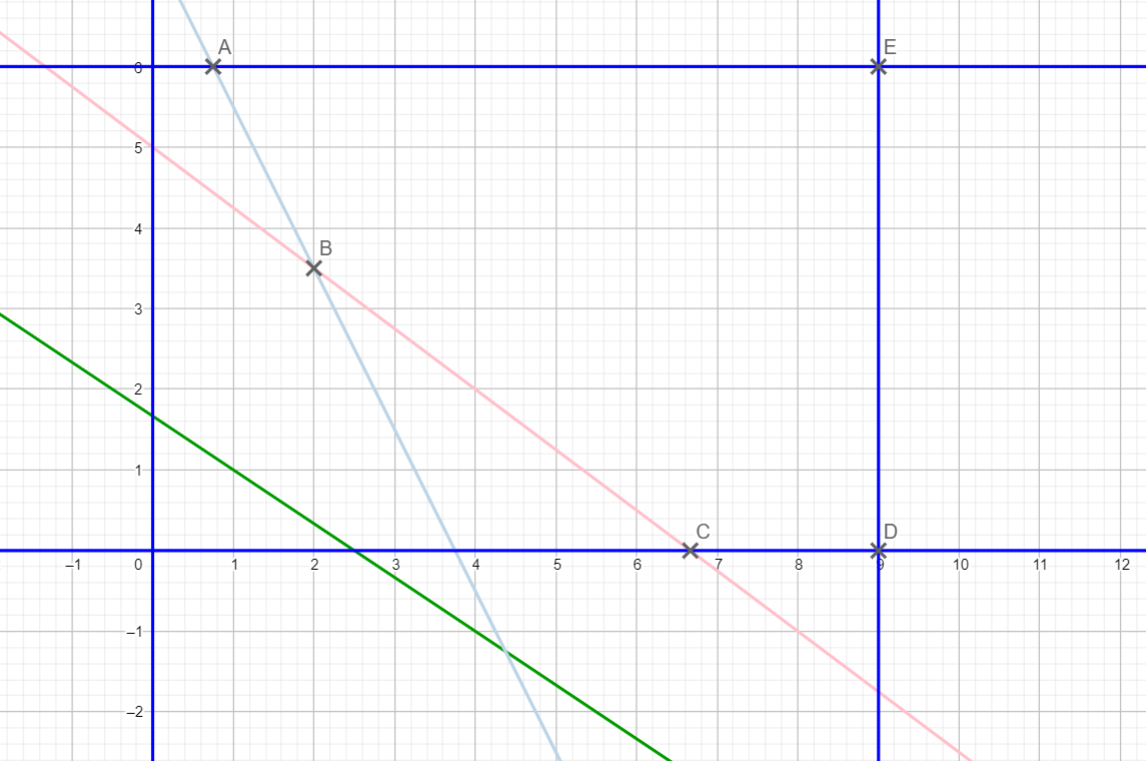
\includegraphics[scale=0.2]{s/imagen.png}
                \\
            en donde el área definida entre los puntos: $A$,$B$,$C$,$D$,$E$ es la región factible y tenemos que el eje de las abscisas es $x_1$ y el de las ordenadas $x_2$
    \item Determina si la región de soluciones factibles es o no acotada.\\
    
            Como se puede ver el area definitivamente se encuentra acotada bajo cualquier punto fuera de la figura definida por $A$,$B$,$C$,$D$,$E$
    \item Identifica los puntos extremos de la región de soluciones factibles.\\
    
        Como vemos los puntos factibles son los siguientes y estan definidos por:\\
         $$A={0.4x_1+0.2x_2&= 1.5} & \cap {x_2=6}=(0.75,6)$$
         $$B={0.3x_1+0.4x_2&=2} & \cap {0.4x_1+0.2x_2&= 1.5}=(2,3.5) $$
         $$C={0.3x_1+0.4x_2&=2} & \cap {x_2=0}=(\frac{20}{3},0)$$
         $$D={x_2=0} & \cap{x_1=9}=(9,0)$$
         $$E={x_1=9} & \cap{x_2=6}=(9,6)$$
    \item Aplica el teorema correspondiente de los vistos en clase, para encontrar el valor mínimo de la función objetivo.\\
    Evaluando cada uno de los puntos obtenidos obtenemos la siguiente tabla:
\begin{table}[h]
\begin{tabular}{@{}llll@{}}
\toprule
Punto & $x_{1}$ & $x_{2}$ & Función objetivo \\ \midrule
A     & 0.75    & 6    & 105    \\
B     & 2    & 3.5  & 92.5      \\
C     & $\frac{20}{3}$ & 0    & 133.33333   \\
D     & 9    & 0    & 180   \\
E     & 9    & 6    & 270   \\ \bottomrule

y como podemos ver la solución para nuestra función objetivo es $B=(2, 3.5)$
\end{tabular}
\end{table}
\end{itemize}

\end{document}
